%%%%%%%%%%%%%%%%%%%%%%%%%%%%%%%%%%%%%%%%%
% Short Sectioned Assignment
% LaTeX Template
% Version 1.0 (5/5/12)
%
% This template has been downloaded from:
% http://www.LaTeXTemplates.com
%
% Original author:
% Frits Wenneker (http://www.howtotex.com)
%
% License:
% CC BY-NC-SA 3.0 (http://creativecommons.org/licenses/by-nc-sa/3.0/)
%
%%%%%%%%%%%%%%%%%%%%%%%%%%%%%%%%%%%%%%%%%

%----------------------------------------------------------------------------------------
%	PACKAGES AND OTHER DOCUMENT CONFIGURATIONS
%----------------------------------------------------------------------------------------

\documentclass[paper=A4, fontsize=11pt]{scrartcl} % A4 paper and 11pt font size

\usepackage[T1]{fontenc} % Use 8-bit encoding that has 256 glyphs
\usepackage[english]{babel} % English language/hyphenation
\usepackage{amsmath,amsfonts,amsthm} % Math packages
\usepackage{tikz} % to graph
\tikzset{
  treenode/.style  	= 	{shape=rectangle, rounded corners,
                     	draw, align=center,
                     	top color=white, bottom color=blue!20},
  predicat/.style  	= 	{treenode, bottom color=red!30},
  conclusion/.style	= 	{treenode},
}
\usepackage{sectsty} % Allows customizing section commands
\usepackage{url}

\allsectionsfont{\centering \normalfont\scshape} % Make all sections centered, the default font and small caps


\usepackage{graphicx}
\usepackage{fancyhdr} % Custom headers and footers
\pagestyle{fancyplain} % Makes all pages in the document conform to the custom headers and footers
\fancyhead{} % No page header - if you want one, create it in the same way as the footers below
\fancyfoot[L]{} % Empty left footer
\fancyfoot[C]{} % Empty center footer
\fancyfoot[R]{\thepage} % Page numbering for right footer
\renewcommand{\headrulewidth}{0pt} % Remove header underlines
\renewcommand{\footrulewidth}{0pt} % Remove footer underlines
\setlength{\headheight}{13.6pt} % Customize the height of the header

%\numberwithin{equation}{section} % Number equations within sections (i.e. 1.1, 1.2, 2.1, 2.2 instead of 1, 2, 3, 4)
%\numberwithin{figure}{section} % Number figures within sections (i.e. 1.1, 1.2, 2.1, 2.2 instead of 1, 2, 3, 4)
%\numberwithin{table}{section} % Number tables within sections (i.e. 1.1, 1.2, 2.1, 2.2 instead of 1, 2, 3, 4)

\setlength\parindent{0pt} % Removes all indentation from paragraphs - comment this line for an assignment with lots of text


%----------------------------------------------------------------------------------------
%	TITLE SECTION
%----------------------------------------------------------------------------------------

\newcommand{\horrule}[1]{\rule{\linewidth}{#1}} % Create horizontal rule command with 1 argument of height

\title{	
\normalfont \normalsize 
\textsc{Johns Hopkins University - Database} \\ [25pt] % Your university, school and/or department name(s)
\horrule{0.5pt} \\[0.4cm] % Thin top horizontal rule
\huge Automatic and periodical data extractions for some NBA aggregate statistics \\ % The assignment title
\horrule{2pt} \\[0.5cm] % Thick bottom horizontal rule
}

\author{Nikhil Panu (415), Gilbert Maystre (415)} % Your name

\date{\normalsize\today} % Today's date or a custom date

\begin{document}

\maketitle % Print the title
\newpage
%----------------------------------------------------------------------------------------
%	PROBLEM 1
%----------------------------------------------------------------------------------------
\section{Overview}
In this project, we focused on building a server that will fetch data smartly from NBA.com and use the induced temporality in the data to plot some aggregate statistics.

\section{Data URL}

TODO: Nik (put where is the source of data). For a more precise text, please refer to the "Fetching the data" section.

\section{Running our code}
We wrote our code in java and python. The java parts call's the python code implicitly, so no need to do anything. The java parts has two main. The first, in class Bootstrap.java is the server side of our app. It launches the services that fills the database. The second main is to be found in Analyzer.java, it's job is to query the database and plot stem graphs. 

Analyzer.java comes precompiled as a jar file you can simply double click on it or type in \verb!java -jar Analyzer.jar!. The actual database should be put exactly as:

\begin{verbatim}
<folder where the jar is>/data/db.sql
\end{verbatim}

Those two files comes in the runnable folder of the archive.

\section{Specialization}

\subsection{Fetching the data}
TODO: Nik

\subsection{Designing a GUI to render temporality}
Since we fetch the data in a periodical fashion, we can get nice stem plots. On the x-axis lies the time, and on the y axis lies the aggregate statistic. This can show new hidden relations in data such as: "Does this particular player do better on week-end games?"\\

Sometimes, simplicity is good. We decided to make only one query available but to make it parametrizable via combo boxes (see Figure \ref{sc1}, \ref{sc2}). The advantage of using combo boxes is that it prevents SQL injections problems and that it clearly shows the user was the program has to offer.\\

We coded the GUI from scratch with only \verb!Java.Swing! API.

\begin{figure}[h]
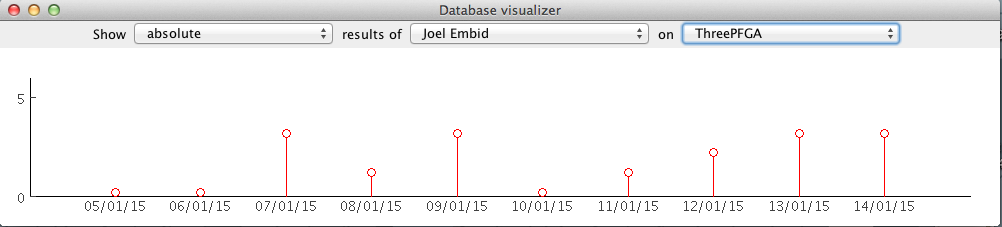
\includegraphics[scale=0.4]{sc1.png}
\centering
\caption{Our GUI with some data}
\label{sc1}
\end{figure}

\begin{figure}[h]
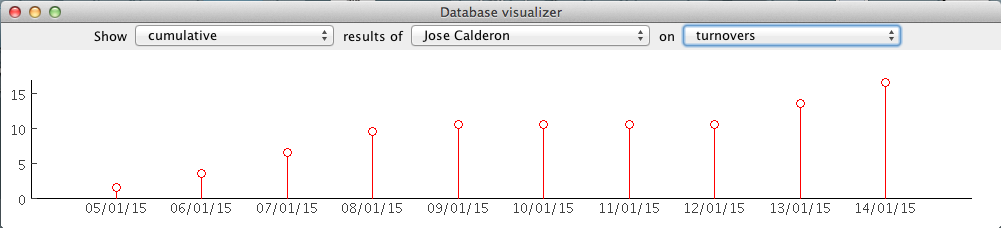
\includegraphics[scale=0.4]{sc2.png}
\centering
\caption{Our GUI with some data and another query.}
\label{sc2}
\end{figure}

\section{Limitation and further improvements}
TODO: fill the data fetching part Niki.\\

On the GUI part, we could quite easily add more feature and queries. This would not require much time, but the point of this executable was to show that it was possible.

\section{Description of the database}
TODO: Niki

\newpage

\section{All SQL code}
We did not use extensively SQL since the goal of our project was mainly to fetch data smartly, but those are the queries our program uses.

\subsection{Constructing the database}
(From \verb!SQLStorer.prepareCuteDatabase()!.)

\begin{verbatim}
CREATE TABLE IF NOT EXISTS Player(FName TEXT, LName TEXT, Age Integer,
   Height DECIMAL(5, 2), Weight DECIMAL(5, 2), Years_Pro Integer, 
   Position TEXT, PRIMARY KEY (FName, LName))
        
CREATE TABLE IF NOT EXISTS Statistics(FName TEXT, LName TEXT,
   TimeStep Integer, Games_Played Integer, Points Integer, Rebounds Integer,
   Assists Integer, Steals Integer, Blocks Integer, Turnovers Integer, FGM Integer,
   ThreePFGM Integer, FGA Integer, ThreePFGA Integer, FTM Integer, FTA Integer,
   PRIMARY KEY(FName, LName, TimeStep))
        
CREATE TABLE IF NOT EXISTS Team(TeamName TEXT, Location TEXT, Conference TEXT,
   Division TEXT, Wins Integer, Losses Integer, PRIMARY KEY(TeamName))
        
CREATE TABLE IF NOT EXISTS PlaysFor(FName TEXT, LName TEXT, TeamName TEXT,
   PRIMARY KEY(FName, LName, TeamName))
        
CREATE TABLE IF NOT EXISTS Date(TimeStep Integer, Date TEXT, PRIMARY KEY(TimeStep))
\end{verbatim}

\subsection{Inserting fetched data}
(From various methods in \verb!SQLStorer.java!.) All the parameters starting with ":" are binded after some kind of processing to avoid SQL injection.

\begin{verbatim}
INSERT INTO Player Values(:FName, :LName, :Age, :Height, :Weight, :Years_Pro,
   :Position)
                
INSERT INTO Team Values(:TeamName, :Location, :Conference, :Division, :Wins,
   :Losses)
                            
INSERT INTO PlaysFor Values(:FName, :LName, :TeamName)
                                        
INSERT INTO Statistics Values(:FName , :LName, :TimeStep, :Games_Played,
   :Points, :Rebounds, :Assists, :Steals, :Blocks, :Turnovers, :FGM, :ThreePFGM,
   :FGA, :ThreePFGA, :FTM, :FTA)
                    
INSERT INTO Date Values(:TimeStep , :Date)
                            
SELECT max(timestep) as u FROM Statistics
                                    
SELECT * FROM Player
\end{verbatim}

\subsection{Fetching the database}
(From various methods in \verb!WrapperUtility.java!).

\begin{verbatim}
SELECT P.FName, P.LName FROM Player as P
        
SELECT D.Date, S.<attribute> 
FROM Statistics as S, Date as D 
WHERE S.FName = :FName AND S.LName = :LName AND D.TimeStep = S.TimeStep
        
SELECT max(S."+attribute+") as m FROM Statistics as S                
\end{verbatim}

\end{document}
